\chapter{Sprechen}

\section{Stichworte zur Vorlesung \em{Artikulatorische Phonetik}} 

Sprechen als aerodynamischer Prozess, Kehlkopf/Larynx, Stimmlippen(schwingung), Phonation, Vokaltrakt... $\rightarrow$ {\tt L2\underline{\ }Artikulation.pdf}

\begin{figure}[htbp]
\begin{center}
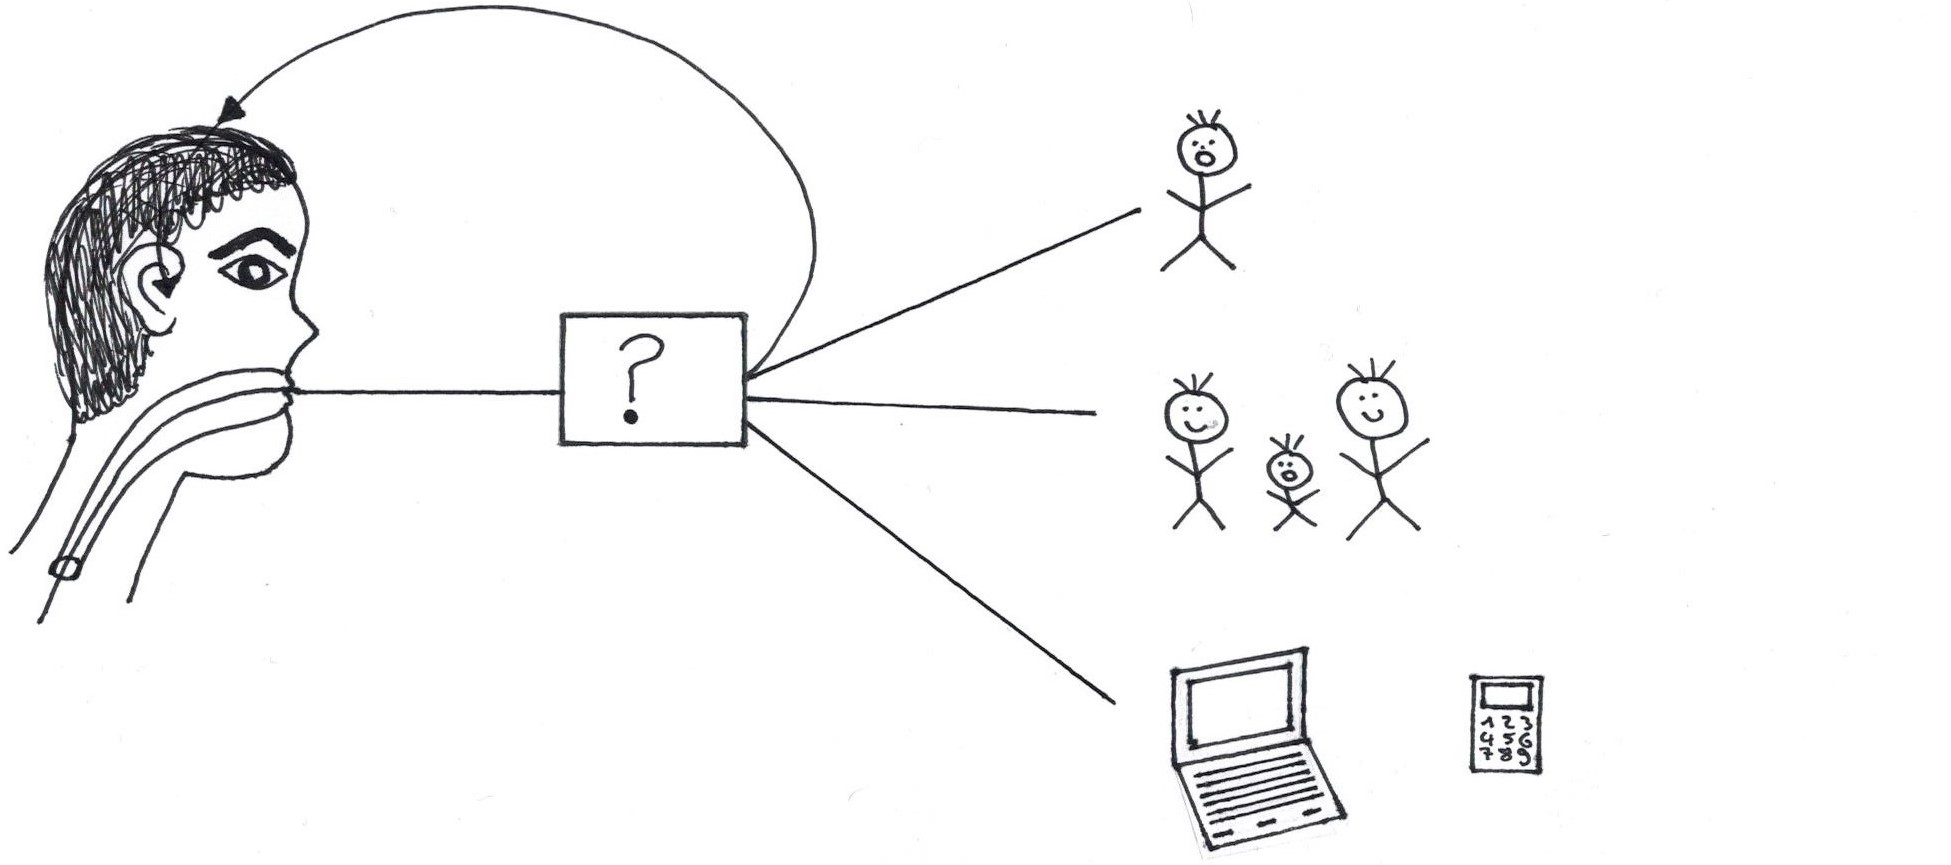
\includegraphics[width=\textwidth]{grafiken/sprechen/sprechen.jpg}
\label{t1}
\end{center}
\end{figure}



\section{Übungen}

1.	Wie viele Sprachlaute gibt es ihrer Meinung nach im Deutschen? Listen Sie sie auf und notieren Sie Beispielwörter, in denen diese vorkommen.
\vspace*{7cm}


2. Beschriften Sie bitte die nachfolgende Abbildung.
\begin{figure}[htbp]
\begin{center}
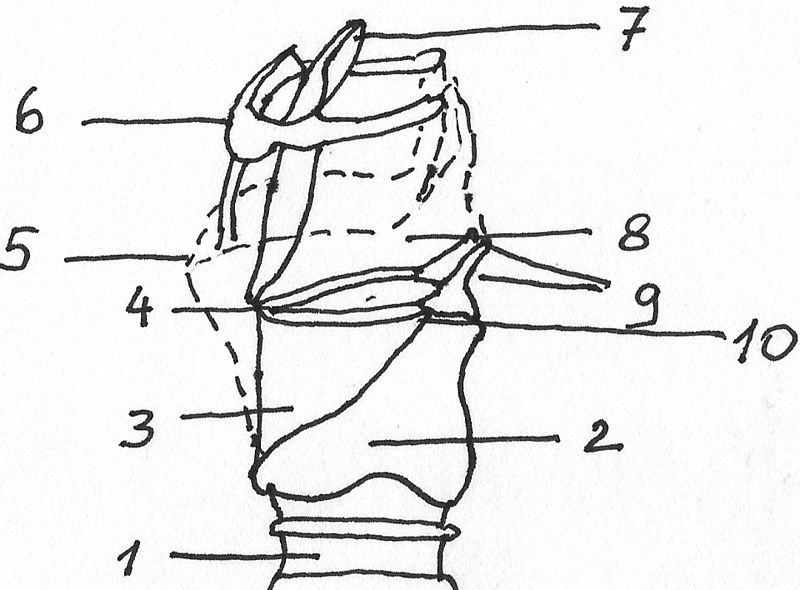
\includegraphics[scale=3]{grafiken/sprechen/kehlkopf.jpg}
\caption{Kehlkopf}
\label{fig2}
\end{center}
\end{figure}

\newpage
3.	Benennen Sie die nummerierten Bereiche des nachfolgend abgebildeten Vokaltraktes:
\begin{figure}[htbp]
\begin{center}
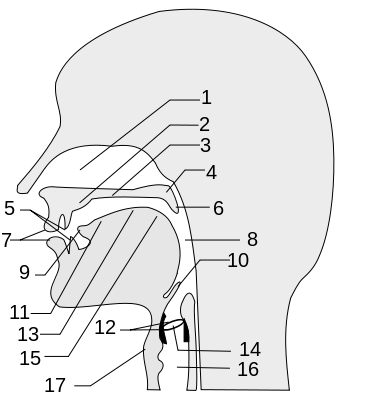
\includegraphics[scale=0.6]{grafiken/sprechen/kopf.png}
\caption{©  Tavin /Wikimedia Commons / CC-BY-3.0}
\label{fig3}
\end{center}
\end{figure}

4.	Welche Sprechorgane neben den Stimmlippen haben aerodynamische Funktionen?
\begin{figure}[htbp]
\begin{center}
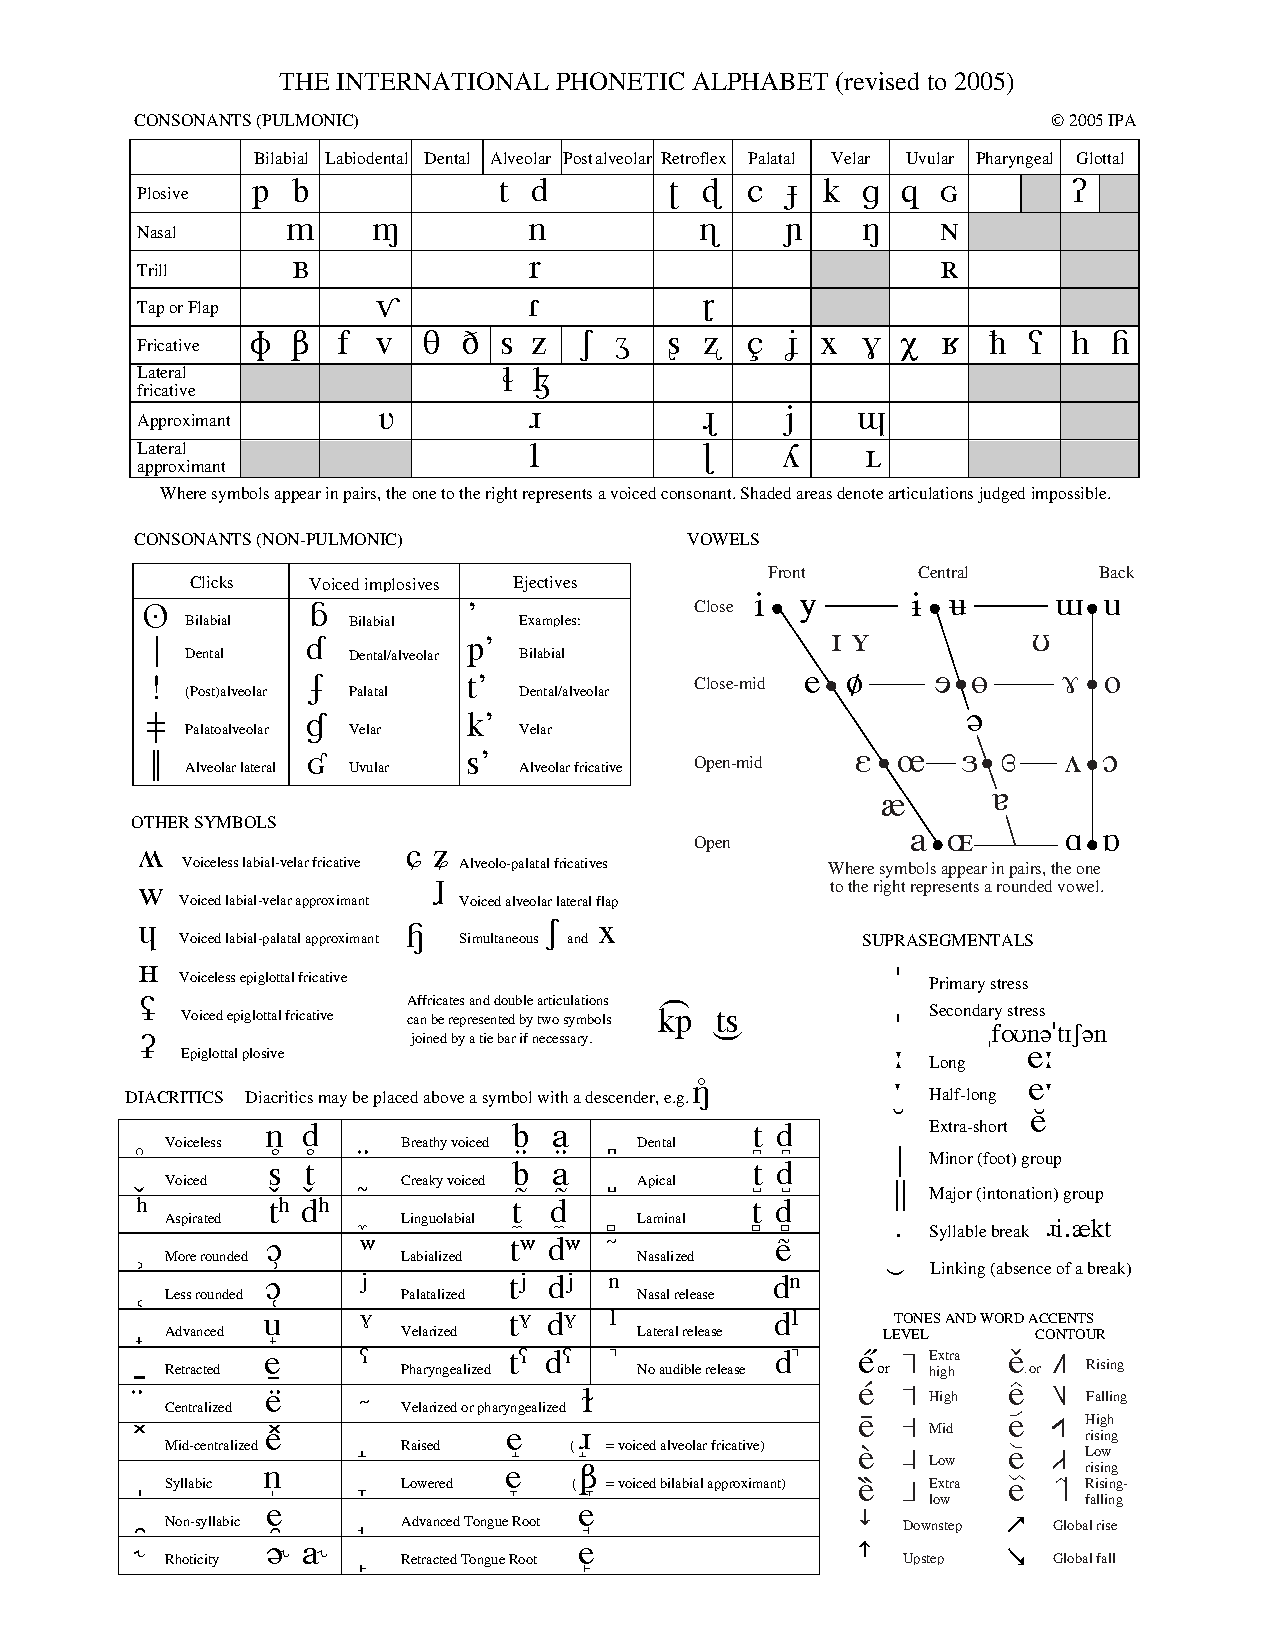
\includegraphics[width=\textwidth]{grafiken/sprechen/ipa.pdf}
\caption{IPA-Tabelle}
\label{fig4}
\end{center}
\end{figure}
